The goal of this section is two-fold: first, we illustrate the computational
efficiency of the two-level method, and second, we verify the theoretical rates
of convergence developed in \autoref{sse:SQGE2LE}.  To illustrate the
computational efficiency of the two-level method, we compare solution times for
the full nonlinear one-level problem and for the two-level method applied to the
SQGE. We choose coarse mesh/fine mesh pairs such that the ratio is
$\nicefrac{1}{2}$. To verify the theoretical rates of convergence, we compare
the theoretical error estimates to the observed rates of convergence from our
numerical tests. For the one-level problem we rely on our original code that was
benchmarked in \cite{Foster}.

To this end we apply the two-level method to the SQGE \eqref{eqn:SQGE_Psi}
with $Re=Ro=1$ and exact solution
\begin{equation}
  \psi(x,y) = \left(\sin 4\pi x \cdot \sin 2\pi y\right)^2.
  \label{eqn:2LExact}
\end{equation}
Additionally, the homogeneous boundary conditions are $\psi=\dfrac{\partial
\psi}{\partial \mathbf{n}}=0$ and the forcing function $F$ corresponds to the exact
solution \eqref{eqn:2LExact}. These boundary conditions and exact solution will
be used in all the two-level tests that follow.

\subsection{Practical Consideration}
A key part of two-level algorithms is accessing a previous coarse mesh solution,
i.e. finding the parent element given a child element. This step can negate any
performance benefits if not implemented wisely. Indeed, let $ n $ be the number
of elements in the FE discretization. For the unit square, a na\"{i}ve search
across every element takes $ O(n/2) $ operations. This procedure may be improved
with a binary search, which is summarized in \autoref{alg:TwoLevelLookup}.

We note that every element on the fine mesh corresponds to exactly one element
on the coarse mesh. However, a coarse mesh element may correspond to multiple
elements on the fine mesh.

\begin{algorithm}%[H]
  \caption{ Given an element on the fine mesh determine the parent element on
  the coarse mesh.}
  \label{alg:TwoLevelLookup}
  Before examining the fine mesh, sort the coarse mesh elements by their
  centroid values.
  \begin{enumerate}[Step 1:]
    \item Select an element on the fine mesh and compute its centroid.
    \item Perform a binary search across the coarse mesh elements until
      the difference between the $ x $-values of the fine mesh centroid
      and coarse mesh centroids is less than $ H $, the coarse mesh step
      size. There should be many elements that fit this condition; save
      them as a list.
    \item Search through this list until we find the correct coarse mesh
      element (that is, the centroid of the fine-mesh element is an
      interior point of the correct coarse mesh element).
  \end{enumerate}
\end{algorithm}

For the considered unit square, the binary search will examine on average
$\log(n)$ elements, while the linear search component involves at most
$\sqrt{n}/2$ elements. Therefore the search requires a $O(\sqrt{n}/2)$ number of
element checks. Profiling results indicate that using
\autoref{alg:TwoLevelLookup} to identify parent elements takes much less time
than either setting up or solving the systems, so this approach is fast enough
that lookup time does not contribute significantly to overall solution time.

\subsection{Computational Efficiency}\label{sse:Efficiency}
To illustrate the computational efficiency of the two-level method, we compare
the simulation time for the standard one-level method (i.e. the full nonlinear
system, without the two-level method) with the simulation time for the two-level
method.

In \autoref{tab:Efficiency}, the $L^2$-norm of the error ($e_{L^2}$), the
$H^2$-norm of the error ($e_{H^2}$) and the simulation times are listed for
various mesh sizes. For each fine mesh, we choose a coarse mesh that ensures the
same order of magnitude for the errors in the one-level and two-level methods.
For small values of the fine mesh size, $h$, the two-level method was
significantly faster than the one-level method. The errors in the $H^2$-norm
were nearly identical, while the error in the $L^2$-norm were generally of the
same order of magnitude. We also note that the tolerance in Newton's method
seems to cause a plateau in the $L^2$-norm of the error. The results in
\autoref{tab:Efficiency} are illustrated graphically in
\autoref{fig:Efficiency}. In this figure the simulation times of the one-level
method (green) and of the two-level method (blue) are displayed for all the
pairs $(h,H)$ in \autoref{tab:Efficiency}.  \autoref{fig:Efficiency} clearly
shows that as the number of degrees of freedom (DoFs) increases, the
computational efficiency of the two-level method increases as well.


\begin{table}
  \begin{center}
    {\small
    \begin{tabular}{|c|c|c|c|c|c|c|}
      \hline
        $H$ & $h$    & DoFs, $H$ & DoFs, $h$ & $e_{L^2}$ & $e_{H^2}$ & time, $s$ \\[0.2em]
      \hline
      $-$         & $0.05146$   & $-$       & $4362$    & $4.29\times 10^{-8}$
        & $1.65\times 10^{-3}$ & $3.328$ \\[0.2em]
      $0.1083$    & $0.05146$   & $1158$    & $4362$    & $1.09\times 10^{-7}$
        & $1.71\times 10^{-3}$            & $2.372$ \\[0.2em]
      $-$         & $0.02561$   & $-$       & $16926$   & $5.75\times 10^{-10}$
        & $1.01\times 10^{-4}$ & $19.92$ \\[0.2em]
      $0.05146$   & $0.02561$   & $4362$    & $16926$   & $7.69\times 10^{-10}$
        & $1.02\times 10^{-4}$           & $11.82$ \\[0.2em]
      $-$         & $0.01597$   & $-$       & $43074$   & $4.75\times 10^{-11}$
        & $1.79\times 10^{-5}$ & $55.69$ \\[0.2em]
      $0.03384$   & $0.01597$   & $10983$   & $43074$   & $5.27\times 10^{-11}$
        & $1.80\times 10^{-5}$ & $33.19$ \\[0.2em]
      $-$         & $0.01277$   & $-$       & $66678$   & $8.66\times 10^{-12}$
        & $6.21\times 10^{-6}$ & $102.4$ \\[0.2em]
      $0.02561$   & $0.01277$   & $16926$   & $66678$   & $9.69\times 10^{-12}$
        & $6.22\times 10^{-6}$ & $59.03$ \\[0.2em]
      $-$         & $0.009659$  & $-$       & $116614$  & $3.88\times 10^{-12}$
        & $2.38\times 10^{-6}$ & $161.7$ \\[0.2em]
      $0.02035$   & $0.009659$  & $29501$   & $116614$  & $6.84\times 10^{-12}$
        & $2.39\times 10^{-6}$ & $95.93$ \\[0.2em]
      $-$         & $0.007959$  & $-$       & $170598$  & $4.79\times 10^{-12}$
        & $1.11\times 10^{-6}$ & $325.1$ \\[0.2em]
      $0.01597$   & $0.007959$  & $43074$   & $170598$  & $9.09\times 10^{-12}$
        & $1.11\times 10^{-6}$ & $172.3$ \\[0.2em]
      $-$         & $0.006854$  & $-$       & $230574$  & $1.79\times 10^{-11}$
        & $6.16\times 10^{-7}$ & $401.7$ \\[0.2em]
      $0.01436$   & $0.006854$  & $58131$   & $230574$  & $1.30\times 10^{-11}$
        & $6.16\times 10^{-7}$ & $219.5$ \\[0.2em]
      $-$         & $0.006374$  & $-$       & $264678$  & $3.91\times 10^{-11}$
      & $3.85\times 10^{-7}$ & $559.7$ \\[0.2em]
      $0.01277$   & $0.006374$  & $66678$   & $264678$  & $2.31\times 10^{-11}$
        & $3.89\times 10^{-7}$ & $291.9$\\[0.2em]
      $-$         & $0.005264$  & $-$       & $389994$  & $3.85\times 10^{-11}$
        & $2.09\times 10^{-7}$ & $753.4$ \\[0.2em]
      $0.01101$   & $0.005264$  & $98133$   & $389994$  & $6.50\times 10^{-11}$
        & $2.09\times 10^{-7}$ & $397.7$ \\[0.2em]
      \hline
    \end{tabular}}
  \end{center}
  \caption{Comparison of one-level and two-level methods: the $L^2$-norm of the
    error ($e_{L^2}$), the $H^2$-norm of the error ($e_{H^2}$) and simulation
    times.}
  \label{tab:Efficiency}
\end{table}

\begin{center}
  \begin{figure}
    \begin{center}
    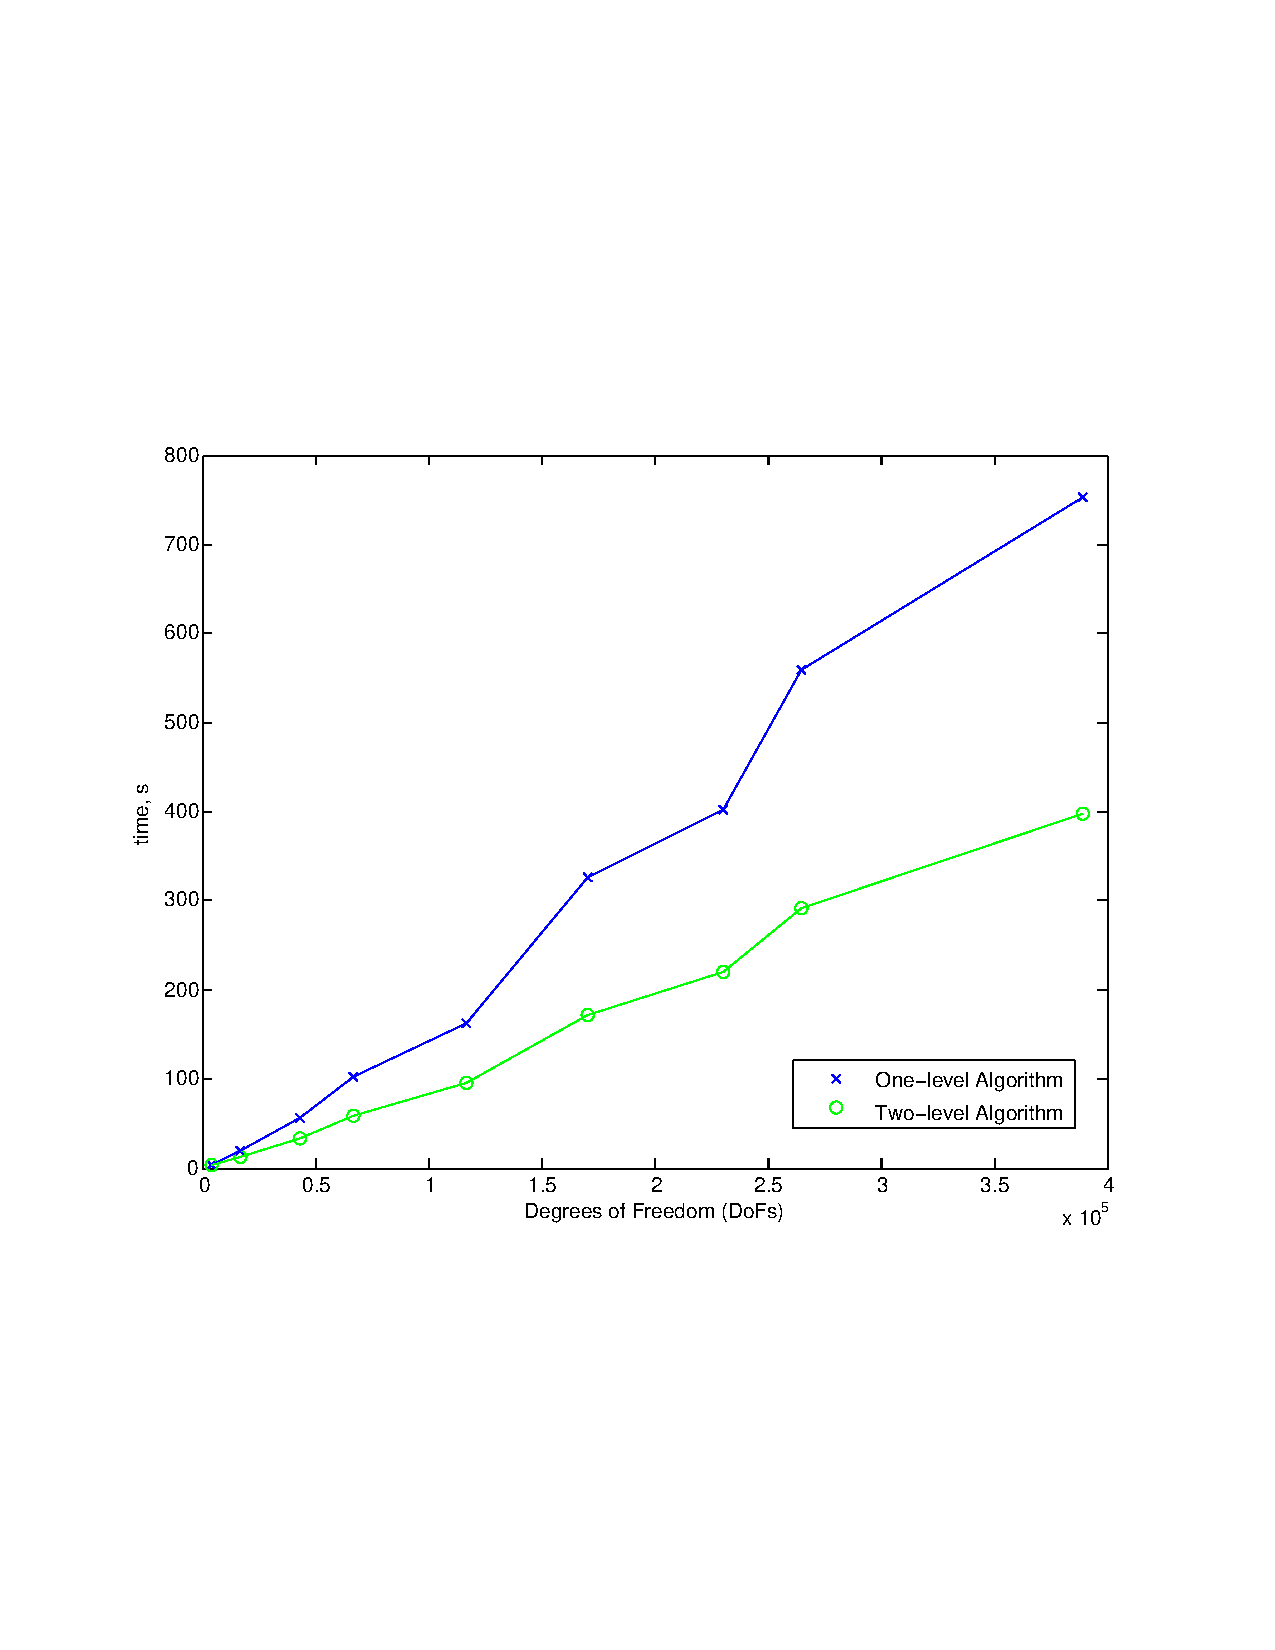
\includegraphics[width=4in,natwidth=610,natheight=642]{Figures/performanceplot.pdf}
    \caption{The simulation times of the one-level method (green) and of the
      two-level method (blue) are displayed for all the pairs $(h,H)$ in
      \autoref{tab:Efficiency}.}
    \label{fig:Efficiency}
    \end{center}
  \end{figure}
\end{center}

\subsection{Rates of Convergence}\label{sse:Rates}
The goal of this subsection is to verify, numerically, the theoretical rates of
convergence in \eqref{eqn:TwoLevelError} of Corollary \ref{crl:Argyris2L}. Unlike
the theoretical error estimates for the one-level method developed in
\cite{Foster}, for the two-level method we must verify rates of convergence
for two different meshes: the fine mesh, $h$, and the coarse mesh, $H$.

To verify, numerically, the theoretical rate of convergence with respect to $H$,
given in \eqref{eqn:TwoLevelError}, we fix $h$ to a small value and we vary $H$.
Thus, the total error in \eqref{eqn:TwoLevelError} will be dominated by the $H$
term, i.e. the total error will of order $O(H^5)$. In \autoref{tab:TwoLevelH},
we fix $h=0.0063$ and we vary $H$. The error in the $L^2$-norm ($e_{L^2}$), the
error in the $H^2$-norm ($e_{H^2}$), and the rate of convergence with respect to
$H$ are listed in \autoref{tab:TwoLevelH}. The rate of convergence follows the
theoretical rate predicted in \eqref{eqn:TwoLevelError} (i.e. fifth-order). For the
last mesh pair, however, the rate of convergence appears to drop off. This
occurs because, for small values of $H$, the total error in
\eqref{eqn:TwoLevelError} is not dominated anymore by the $H$ term.
\begin{table}
  \begin{center}
    \begin{tabular}{|c|c|c|c|c|c|c|}
    \hline
      $H$ &   $h$ &   DoFs, $ H $ & DoFs, $ h $ & $e_{H^2}$ & $H^2$ order \\
      \hline
      $0.43$ & $0.0063$ & $350$ & $296710$ & $4.54\times 10^{-1}$ & $-$ \\[0.2em]
      $0.21$ & $0.0063$ & $1270$ & $296710$ & $1.75\times 10^{-2}$ & $4.45$ \\[0.2em]
      $0.10$ & $0.0063$ & $4838$ & $296710$ & $4.92\times 10^{-4}$ & $5.04$ \\[0.2em]
      $0.05$ & $0.0063$ & $18886$ & $296710$ & $1.32\times 10^{-5}$ & $5.20$ \\[0.2em]
      $0.025$ & $0.0063$ & $74630$ & $296710$ & $6.02\times 10^{-7}$ & $4.45$ \\[0.2em]
      \hline
    \end{tabular}
  \end{center}
  \caption{Observed order of convergence in the $H^2$ norm for the coarse mesh,
    $H$, in the Two-level method applied to \eqref{eqn:QGE_psi} with exact
    solution \eqref{eqn:2LExact}.}
  \label{tab:TwoLevelH}
\end{table}

\begin{figure}
  \begin{center}
    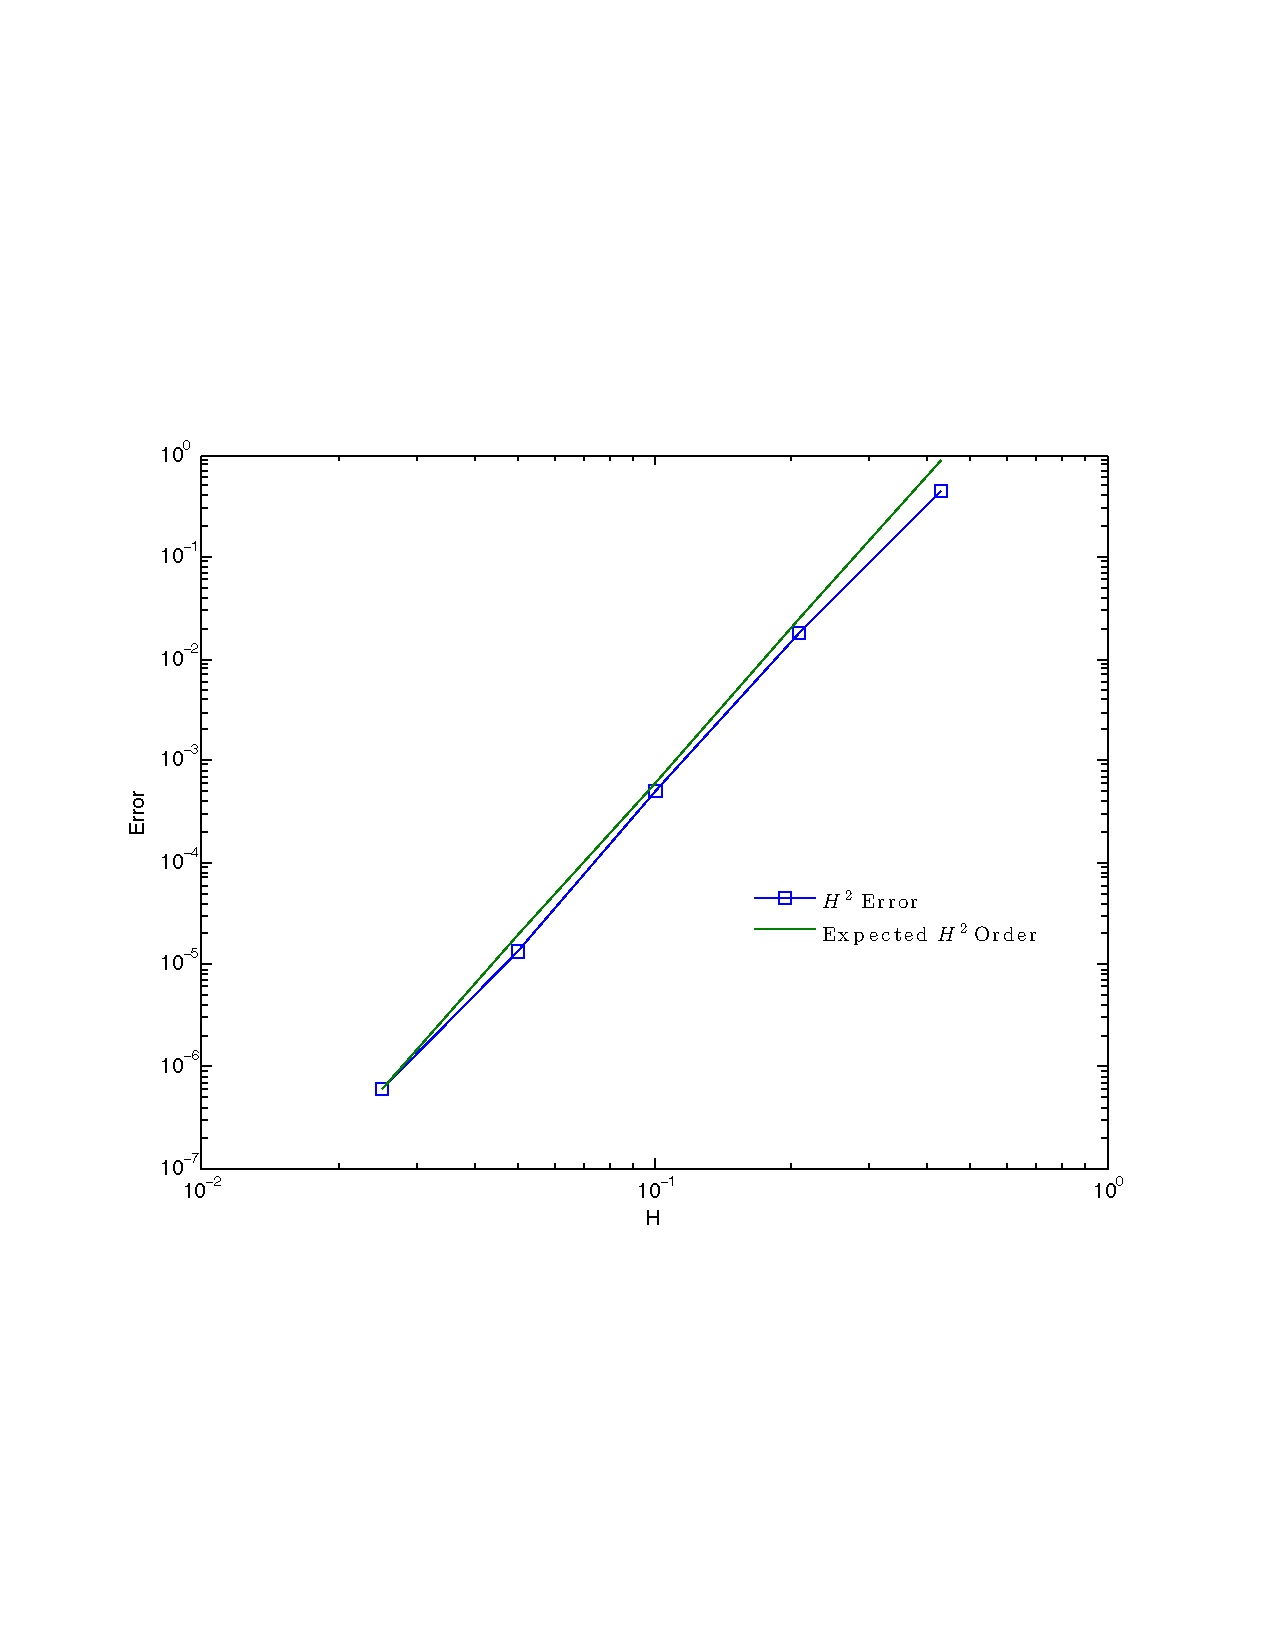
\includegraphics[scale=0.6]{Figures/CoarseConvergence.pdf}
    \caption{Observed order of convergence in the $H^2$ norm for the coarse
      mesh, $H$, in the Two-Level method applied to \eqref{eqn:QGE_psi} with the
      exact solution \eqref{eqn:2LExact}.}
  \label{fig:TwoLevelH}
  \end{center}
\end{figure}

To verify, numerically, the theoretical rate of convergence with respect to
$h$, given in \eqref{eqn:TwoLevelError}, we must proceed with caution. The reason is
that a straightforward approach would fix $H$ and let $h$ go to zero. This
approach, however, would fail, since the $H$ term would eventually dominate the
total error. To avoid this, we consider the following scaling between the mesh
sizes:
\begin{equation}
  H = C\, h,
  \label{eqn:C-Scaling}
\end{equation}
where $C>1$. The scaling in \eqref{eqn:C-Scaling} implies that the total error
in \eqref{eqn:TwoLevelError} is of order $O(h^4)$. Indeed, the second term on the
right hand side of \eqref{eqn:TwoLevelError} now scales as follows:
\begin{equation}
  \begin{split}
    C_2 \sqrt{|\ln(h)|}\, H^5 &\approx C_2 C \sqrt{|\ln(h)|}\, h^5 \\[0.2em]
    \approx O(h^4),
  \end{split}
  \label{eqn:Balance}
\end{equation}
where in the last relation in \eqref{eqn:Balance} we used the fact that
$\sqrt{|\ln(h)|}\, h \rightarrow 0$ when $h \rightarrow 0$ (which follows from
l'Hospital's rule).

\begin{remark}
  We emphasize that the scaling in \eqref{eqn:C-Scaling} is not needed in the
  two-level algorithm. We only use it in this subsection to monitor the
  convergence rate with respect to $h$.
\end{remark}

In this subsection, we consider $C=2$ in \eqref{eqn:C-Scaling}. We note,
however, that any other constant $C>1$ could be used in \eqref{eqn:C-Scaling}.
With this choice, we are now ready to verify, numerically, the theoretical rate
of convergence with respect to $h$ given in \eqref{eqn:TwoLevelError}, which, as
shown in \eqref{eqn:Balance}, will be of order $O(h^4)$. In
\autoref{tab:TwoLevelh}, for various mesh size pairs $(H=2h, h)$, we list the
$L^2$-norm of the error ($e_{L^2}$), the $H^2$-norm of the error ($e_{H^2}$),
and the rate of convergence. The rate of convergence follows the theoretical
rate predicted in \eqref{eqn:TwoLevelError} (i.e. fourth-order).

\begin{table}
  \begin{center}
    \begin{tabular}{|c|c|c|c|c|c|c|}
    \hline
      $H$ &   $h$  &  DoFs, $ H $ & DoFs, $ h $ & $e_{H^2}$ & $H^2$ order \\
      \hline
      $1.1$ & $0.43$ & $38$ & $106$ & $5.83\times 10^0$ & $-$ \\[0.2em]
      $0.43$ & $0.21$ & $106$ & $350$ & $6.61\times 10^{-1}$ & $2.56$ \\[0.2em]
      $0.21$ & $0.10$ & $350$ & $1270$ & $3.65\times 10^{-2}$ & $3.96$ \\[0.2em]
      $0.10$ & $0.05$ & $1270$ & $4838$ & $2.00 \times 10^{-3}$ & $4.10$ \\[0.2em]
      $0.050$ & $0.025$ & $4838$ & $18886$ & $1.20\times 10^{-4}$ & $4.04$ \\[0.2em]
      $0.025$ & $0.013$ & $18886$ & $74630$ & $7.40\times 10^{-6}$ & $4.02$ \\[0.2em]
      $0.013$ & $0.0063$ & $74630$ & $296710$ & $4.68\times 10^{-7}$ & $3.99$ \\[0.2em]
    \hline
    \end{tabular}
  \end{center}
  \caption{Observed order of convergence in the $H^2$ norm for the fine mesh,
    $h$, in the Two-Level method applied to \eqref{eqn:QGE_psi} with the exact
    solution \eqref{eqn:2LExact}.}
  \label{tab:TwoLevelh}
\end{table}

\begin{figure}
  \begin{center}
    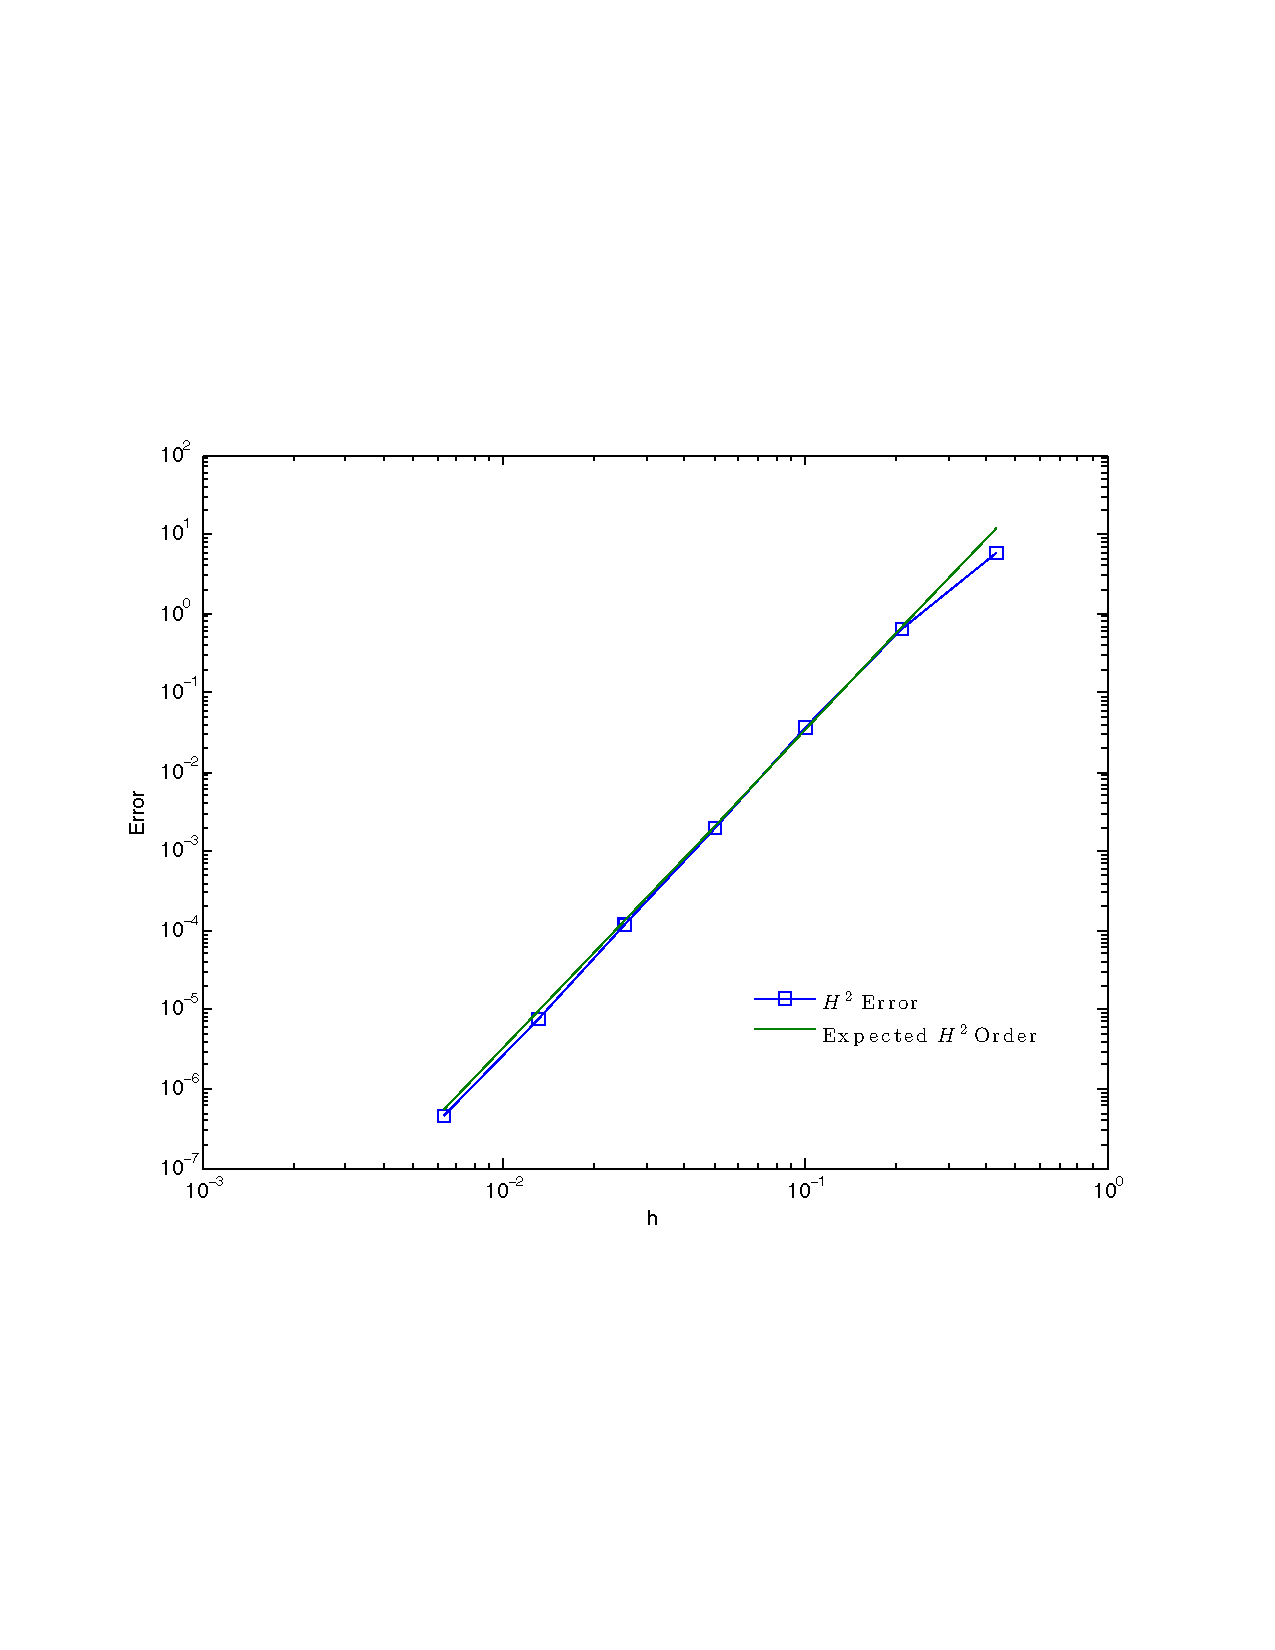
\includegraphics[scale=0.6]{Figures/fineConvergence.pdf}
    \caption{Observed order of convergence in the $H^2$ norm for the fine mesh,
      $h$, in the Two-Level method applied to \eqref{eqn:QGE_psi} with the exact
      solution \eqref{eqn:2LExact}.}
  \label{fig:TwoLevelh}
  \end{center}
\end{figure}
